% $Id: equations.tex 1901 2016-10-13 14:17:41Z uqimccul $
\documentclass{article}
\usepackage{graphicx}
\usepackage{amsmath}
\begin{document}

\newcommand{\deriv}[2]{\frac{\mathrm{d} #1}{\mathrm{d} #2}}
\newcommand{\pderiv}[2]{\frac{\partial #1}{\partial #2}}
\newcommand{\refeq}[1]{Eq.~(\ref{#1})}
\newcommand{\refeqtwo}[2]{Eq.~(\ref{#1},\ref{#2})}
\newcommand{\reffig}[1]{Fig.~(\ref{#1})}

\title{Equations of motion of a bell and clapper}

\author{I. P. McCulloch}
\date{\today}

\maketitle

\section{Notation}

We start by formulating the Lagrangian of a freely swinging bell and clapper. 
The notation is shown in fig \ref{fig:bell}. Let:
\begin{equation}
\begin{array}{rcl}
\theta &=& \mbox{angle of the bell from bottom dead centre} \\
M &=& \mbox{mass of the bell}\\
b &=& \mbox{distance from the axis of the bell to its centre of gravity} \\
I'_b &=& \mbox{moment of inertia of the bell about its centre of gravity} \\
I_b &=& \mbox{moment of inertia of the bell about its axis}\\
K_b &=& \mbox{friction coefficient of the bell}\\
a &=& \mbox{distance from the bell axis to the clapper axis} \\
\alpha &=& \mbox{angle of the clapper axis from the centre line of the bell}\\
\phi &=& \mbox{angle of the clapper from the centre line of the bell}\\
m &=& \mbox{mass of the clapper}\\
c &=& \mbox{distance from the clapper axis to the clapper centre of gravity}\\
I'_c &=& \mbox{moment of inertia of the clapper about its centre of gravity}\\
I_c &=& \mbox{moment of inertia of the clapper about its axis}\\
K_c &=& \mbox{friction coefficient of the clapper}
\end{array}
\end{equation}

\begin{figure}
\begin{centering}
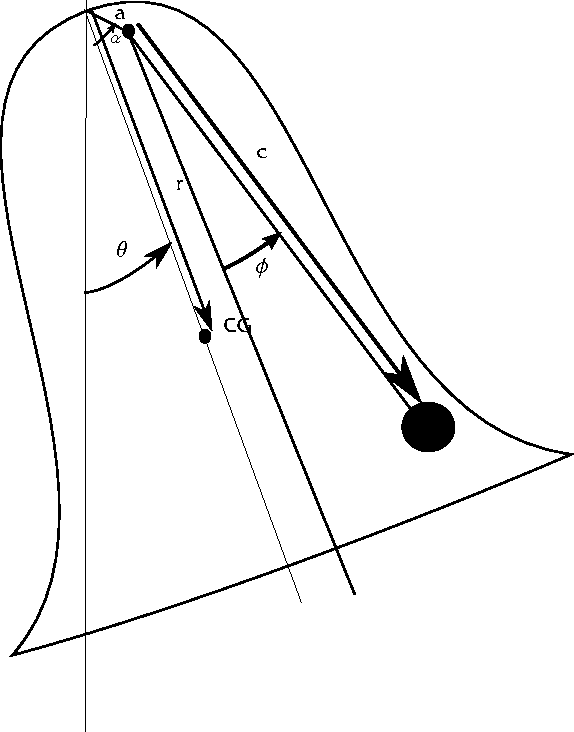
\includegraphics[width=0.8\textwidth]{bellfigure.pdf}\par
\end{centering}
\caption{Notation.  The bell is mass $M$, with centre of gravity located a distance $r$ from
the axis. $\theta$ is the angle of the bell from bottom dead-centre.
The capper has mass $m$, and a pivot axis located at angle $\alpha$ from the centre line of the bell
at a distance $a$ from the bell axis. The clapper has mass $m$ with a centre of gravity located at
a distance $c$ from the clapper axis.  The moment of inertia of the bell about its centre of gravity is
$I'_b$, and of the clapper about its centre of gravity $I'_c$. The moments of inertia of the bell
and clapper about their respective axes are $I_b$ and $I_c$.}
\label{fig:bell}
\end{figure}

Some useful relations follow.  From the parallel axis theorem, 
\begin{equation}
I_b = I'_b + M b^2
\end{equation}
\begin{equation}
I_c = I'_c + m c^2
\end{equation}
To calculate the potential energy it is useful to know the cartesian coordinates of the
bell and clapper. Taking the axis of the bell to be at $(0,0)$, with the usual coodinates the
location of the bell centre of gravity is
\begin{equation}
(b \sin \theta, -b \cos \theta)
\end{equation}
The location of the clapper axis is
\begin{equation}
(a \sin(\theta+\alpha), -a \cos(\theta+\alpha))
\end{equation}
and the clapper centre of gravity is at
\begin{equation}
(a \sin(\theta+\alpha) + c \sin(\theta+\phi), -a \cos(\theta+\alpha) - c \cos(\theta+\phi))
\end{equation}
or, in angular coordinates,
\begin{equation}
\begin{array}{rcl}
r_c^2 &=& a^2 + b^2 + 2ac \cos(\phi - \alpha) \\
\theta_c &=& \theta + \arctan \frac{a \cos \alpha + c \cos \phi}{a \sin \alpha + c \sin \phi}
\end{array}
\end{equation}

\section{Kinetic energy}

The kinetic energy of the bell is the sum of the motion of the centre of gravity plus the rotational
kinetic energy.
\begin{equation}
{KE}_{b} = \frac{1}{2}M r^2 \dot{\theta}^2 + \frac{1}{2}I'_b \dot{\theta}^2 
= \frac{1}{2}I_b \dot{\theta}^2
\end{equation}
To find the kinetic energy of the clapper, we first obtain the velocity in cartesian coordinates
of the clapper centre of mass,
\begin{equation}
\vec{v}_c = (a \dot{\theta} \cos(\theta + \alpha) + c (\dot{\theta} + \dot{\phi}) \cos(\theta+\phi),
a \dot{\theta} \sin(\theta+\alpha) + c (\dot{\theta}+\dot{\phi}) \sin(\theta+\phi))
\end{equation}
which gives the squared velocity
\begin{equation}
v_c^2 = a^2 \dot{\theta}^2 + c^2 (\dot{\theta} + \dot{\phi})^2 
+ 2ac \dot{\theta}(\dot{\theta}+\dot{\phi}) \cos(\phi - \alpha)
\end{equation}
The kinetic energy of the clapper is the sum of the centre of mass motion plus the rotational
kinetic energy about the centre of mass, $m v_c^2/2 + I'_c(\dot{\theta}+\dot{\phi})^2/2$, giving
\begin{equation}
{KE}_{c} = \frac{1}{2}m a^2 \dot{\theta}^2 + \frac{1}{2}I_c (\dot{\theta}+\dot{\phi})^2
+ mac \dot{\theta} (\dot{\theta} + \dot{\phi}) \cos(\phi - \alpha)
\end{equation}
where we have used the parallel axis theorem to use the moment of inertia about the clapper axis.

\section{Potential energy}

We've already obtained the location of the centre of mass of the bell and clapper in cartesian
coordinates so finding the potential energy $mgh$ is straightforwardly, for the bell,
\begin{equation}
{PE}_b = -Mgb \cos \theta
\end{equation}
and
\begin{equation}
{PE}_c = -mg \left(a \cos(\theta+\alpha) + c \cos(\theta + \phi) \right)
\end{equation}
for the clapper.

\section{Lagrangian}

This gives now the Lagrangian for the freely swinging bell+clapper,
\begin{equation}
\begin{array}{rccl}
\cal{L} &=& & I_b \dot{\theta}^2/2 + I_c (\dot{\theta}+\dot{\phi})^2/2 \\
& & + & m a^2 \dot{\theta}^2/2
       + mac \dot{\theta} (\dot{\theta} + \dot{\phi}) \cos(\phi - \alpha) \\
& & + & Mgb \cos \theta + mga \cos(\theta+\alpha) + mgc \cos(\theta + \phi)
\end{array}
\end{equation}

\section{Equations of motion}

We can now obtain Lagrange's equations of motion,
\begin{eqnarray}
\deriv{}{t} \pderiv{\cal{L}}{\dot{\theta}} - \pderiv{\cal{L}}{\theta} &=& 0 \\
\deriv{}{t} \pderiv{\cal{L}}{\dot{\phi}} - \pderiv{\cal{L}}{\phi} &=& 0
\end{eqnarray}

Firstly, for $\theta$, we obtain
\begin{equation}
\pderiv{\cal{L}}{\dot{\theta}} = I_b \dot{\theta} + I_c (\dot{\theta} + \dot{\phi})
+ ma^2 \dot{\theta} 
   + mac (2\dot{\theta} + \dot{\phi}) \cos(\phi-\alpha)
\end{equation}
so that
\begin{equation}
\begin{array}{rcl}
\displaystyle \deriv{}{t} \pderiv{\cal{L}}{\dot{\theta}} &=& I_b \ddot{\theta} + I_c (\ddot{\theta} + \ddot{\phi})
+ ma^2 \ddot{\theta} \\
& & + mac(2 \ddot{\theta} + \ddot{\phi})
\cos(\phi-\alpha) - mac \dot{\phi}(2\dot{\theta} + \dot{\phi}) \sin(\phi - \alpha)
\end{array}
\end{equation}
Now 
\begin{equation}
\pderiv{\cal{L}}{\theta} = 
- Mgb\sin{\theta} - mga \sin(\theta + \alpha) - mgc \sin(\theta + \phi)
\end{equation}
So our equation of motion is
\begin{equation}
\begin{array}{c}
0 = I_b \ddot{\theta} + ma^2 \ddot{\theta} 
+ I_c (\ddot{\theta} + \ddot{\phi}) \\
+ mac(2 \ddot{\theta} + \ddot{\phi}) \cos(\phi-\alpha)
- mac\dot{\phi}(2\dot{\theta} + \dot{\phi}) \sin(\phi - \alpha) \\
+ Mgb\sin{\theta}
+ mga \sin(\theta + \alpha)
+ mgc \sin(\theta + \phi)
\end{array}
\label{eq:motion1}
\end{equation}
Secondly, for $\phi$, we get
\begin{equation}
\pderiv{\cal{L}}{\dot{\phi}} = I_c (\dot{\theta} + \dot{\phi}) + mac \dot{\theta} \cos(\phi - \alpha)
\end{equation}
so that
\begin{equation}
\deriv{}{t} \pderiv{\cal{L}}{\dot{\phi}} = I_c (\ddot{\theta} + \ddot{\phi})
+ mac \ddot{\theta} \cos(\phi - \alpha) - mac \dot{\theta}\dot{\phi} \sin(\phi - \alpha)
\end{equation}
Now
\begin{equation}
\pderiv{\cal{L}}{\phi} = mac \dot{\theta}(\dot{\theta}+\dot{\phi})\sin(\phi - \alpha) 
-mgc \sin(\theta + \phi)
\end{equation}
so that our equation of motion is
\begin{equation}
\begin{array}{c}
0 = I_c (\ddot{\theta} + \ddot{\phi})
+ mac \ddot{\theta} \cos(\phi - \alpha) 
- mac \dot{\theta} \dot{\phi} \sin(\phi - \alpha) \\
+ mac \dot{\theta}(\dot{\theta}+\dot{\phi})\sin(\phi - \alpha) 
+ mgc \sin(\theta + \phi)
\end{array}
\end{equation}
which simplifies to
\begin{equation}
\begin{array}{c}
0 = I_c (\ddot{\theta} + \ddot{\phi})
+ mac \ddot{\theta} \cos(\phi - \alpha) 
+ mac \dot{\theta}^2 \sin(\phi - \alpha)
+ mgc \sin(\theta + \phi)
\end{array}
\label{eq:motion2}
\end{equation}
This is the equation of motion for the clapper. It will be valid only when the
clapper is in free motion, ie when 
\begin{equation}
\phi_1 \leq \phi \leq \phi_2
\end{equation}
where $\phi_1$, $\phi_2$ are the boundary angles at which the clapper strikes the bell.

Our first equation \refeq{eq:motion1} includes several terms in this equation. Hence
we can simplify \refeq{eq:motion1} into
\begin{equation}
\begin{array}{c}
0 = (I_b + ma^2) \ddot{\theta} + mac(\ddot{\theta} + \ddot{\phi}) \cos (\phi - \alpha) \\
-mac (\dot{\theta} + \dot{\phi})^2 \sin(\phi - \alpha)
+ Mgb\sin{\theta}
+ mga \sin(\theta + \alpha)
\end{array}
\label{eq:motion3}
\end{equation}
We take \refeq{eq:motion2} and \refeq{eq:motion3} as our equations of motion.

We will work at simplifying these equations, but firstly lets verify the correctness.
In the special case where $\alpha=0$, $a=b$ (ie, when the clapper axis is located at the
centre of gravity of the bell) this system reduces to a double pendulum. 
Comparing with the Mathworld equations \cite{doublependulum}, we set the notation
\begin{equation}
\begin{array}{rcl}
m_1 &=& M \\
l_1 &=& b \\
\theta_1 &=& \theta \\
m_2 &=& m \\
l_2 &=& c \\
\theta_2 &=& \theta + \phi
\end{array}
\end{equation}
and $I_b = m_1 l_1^2$, $I_c = m_2 l_2^2$. 
Substituting into the equation of motion \refeq{eq:motion2} we obtain
\begin{equation}
\begin{array}{c}
0 = m_2 l_2^2 \ddot{\theta}_2 + m_2 l_1 l_2 \ddot{\theta}_1 \cos(\theta_2 - \theta_1) \\
+ m_2 l_1 l_2 \dot{\theta}_1^2 \sin(\theta_2 - \theta_1)
+ m_2 g l_2 \sin \theta_2
\end{array}
\end{equation}
which is identical to equation (18) of the double pendulum equations at the Wolfram website.
Substituting into the equation of motion
\refeq{eq:motion3} we obtain
\begin{equation}
\begin{array}{c}
0 = (m_1+m_2) l_1^2 \ddot{\theta}_1 + m_2 l_1 l_2 \ddot{\theta}_2 \cos(\theta_2 - \theta_1) \\
- m_2 l_1 l_2 \dot{\theta}_2^2 \sin(\theta_2 - \theta_1) + (m_1+m_2) l_1 g \sin \theta_1
\end{array}
\end{equation}
which coincides with equation (13) of the same reference.

\section{Friction}

We can incorporate friction in the clapper and the bell by modifying Lagrange's equations
to
\begin{eqnarray}
\deriv{}{t} \pderiv{\cal{L}}{\dot{\theta}} - \pderiv{\cal{L}}{\theta} &=& Q_\theta \\
\deriv{}{t} \pderiv{\cal{L}}{\dot{\phi}} - \pderiv{\cal{L}}{\phi} &=& Q_\phi
\end{eqnarray}
where the friction forces are
\begin{eqnarray}
Q_\theta &=& -K_b \dot{\theta} + f(t)\\
Q_\phi &=& -K_c \dot{\phi}
\end{eqnarray}
and we have also added an external force on the bell which will be excerted by the ringer.
This modifies the equations of motion to
\begin{equation}
\begin{array}{c}
0 = K_c \dot{\phi} + I_c (\ddot{\theta} + \ddot{\phi})
+ mac \ddot{\theta} \cos(\phi - \alpha) 
+ mac \dot{\theta}^2 \sin(\phi - \alpha)
+ mgc \sin(\theta + \phi)
\end{array}
\label{eq:motion2friction}
\end{equation}
and, recalling that we derived \refeq{eq:motion3} by subtracting 
\refeq{eq:motion2} from \refeq{eq:motion1}, we obtain
\begin{equation}
\begin{array}{c}
f(t) = K_b \dot{\theta} - K_c \dot{\phi} + (I_b + ma^2) \ddot{\theta} \\
+ mac(\ddot{\theta} + \ddot{\phi}) \cos (\phi - \alpha)
-mac (\dot{\theta} + \dot{\phi})^2 \sin(\phi - \alpha) \\
+ Mgb\sin{\theta}
+ mga \sin(\theta + \alpha)
\end{array}
\label{eq:motion3friction}
\end{equation}

We note that \refeq{eq:motion2friction} is identical (up to a small change of notation) to
that obtained by F.H.~King \cite{king94}. Our equation of motion for the bell 
\refeq{eq:motion3friction} is quite different however, which is due to the fact that we have
allowed the motion of the clapper to influence the bell. In most bells where the clapper is
insignificant to the motion of the bell, which amounts to $mac \ll I_b$, 
and remembering that $K_c$ will be proportional to the mass of the clapper so that is also
negligible, then
\refeq{eq:motion3friction} simplifies quite considerably, to
\begin{equation}
f(t) = K_b \dot{\theta} + I_b \ddot{\theta} + Mgb \sin \theta
\label{eq:bellsimplified}
\end{equation}
which is the same as the equation listed in \cite{king94}. However in situations where
the motion of the clapper does significantly affect the bell, then we must retain all
terms in \refeq{eq:motion3friction}, and also determine what happens when the clapper impacts
with the bell.

\section{Solving the simplified equations}

We now examine what is required to solve the equations \refeq{eq:motion2friction}
and \refeq{eq:bellsimplified}. Following \cite{king94}, let us define
\begin{eqnarray}
l_b &=& \frac{I_b}{Mb} \\
k_b &=& \frac{K_b}{Mb} \\
l_c &=& \frac{I_c}{mc} \\
k_c &=& \frac{K_c}{mc} \\
F(t) &=& \frac{f(t)}{I_b}
\end{eqnarray}
the equations become
\begin{equation}
F(t) = \ddot{\theta} + \frac{k_b}{l_b}\dot{\theta} + \frac{g}{l_b}\sin \theta
\end{equation}
and
\begin{equation}
0=(\ddot{\theta} + \ddot{\phi}) + \frac{k_c}{l_c} \dot{\phi} 
+ \frac{c}{l_c}\ddot{\theta}\cos(\phi-\alpha)
+ \frac{c}{l_c}\dot{\theta}^2 \sin(\phi-\alpha) + \frac{g}{l_c}\sin(\theta+\phi)
\end{equation}
To solve these, we convert into set of coupled first-order equations by introducing
a set of auxiliary variables $v_\theta$ and $v_\phi$. We can solve $\theta$ independently,
\begin{eqnarray}
\dot{\theta} &=& v_\theta \label{eq:dtheta} \\
\dot{v}_\theta &=& F(t) - \frac{k_b}{l_b} v_\theta - \frac{g}{l_b} \sin \theta
\label{eq:vtheta}
\end{eqnarray}
which can be used in an ODE solver.
We can also solve for the clapper position,
\begin{eqnarray}
\dot{\phi} &=& v_\phi \\
\dot{v}_\phi &=& \begin{array}{c}
\dot{v}_\theta \left( 1 + \frac{c}{l_c}\cos(\phi - \alpha) \right) 
- \frac{k_c}{l_c}v_\phi \\
\quad \quad + \frac{c}{l_c} v_\theta^2 \sin(\phi - \alpha) 
+ \frac{g}{l_c}\sin(\theta + \phi)
\end{array}
\end{eqnarray}
Strictly speaking we shouldn't have $\dot{v}_\theta$ on the right hand side, but this is defined
in \refeq{eq:vtheta} anyway.

\section{Pull-ometer}

In the case where the motion of the clapper is insignificant to the motion of the bell, we
need to solve only the pair of first order ODE's \refeqtwo{eq:dtheta}{eq:vtheta}.
If the accelerometer is located at a distance $r$ from the bell axis, 
at an angle $\beta$ from bottom dead centre,
orientated such that the $x$ axis is tangential to the wheel and the $y$ axis is pointing
inwards, then the $x$ axis will measure the angular acceleration plus a component due to gravity,
\begin{equation}
\ddot{x} = r \ddot{\theta} + g \sin (\theta + \beta)
\end{equation}
and the $y$ axis will measure the centripetal acceleration plus gravity,
\begin{equation}
\ddot{y} = -r \dot{\theta}^2 - g \cos (\theta  + \beta)
\end{equation}
Inserting the equations of motion,
\begin{equation}
\ddot{x} = r \left(F(t) - \frac{k_b}{l_b}v_\theta - \frac{g}{l_b}\sin \theta \right) 
   + g \sin (\theta + \beta)
\end{equation}
and
\begin{equation}
\ddot{y} = -r v_\theta^2 - g \cos (\theta  + \beta)
\end{equation}
The idea will be that we solve the equations of motion, which give the instantaneous
$\theta$ and $v_\theta$. To find the time derivatives, we need to know what $F(t)$ is. 
We can calculate that from knowing $\ddot{x}$. But we also know $\ddot{y}$, so we ideally
want to use this to improve the fit. Effectively, we have two equations (for $\ddot{x}$ and
$\ddot{y}$), with three unknowns, $\theta$, $v_\theta$ and $F(t)$. 

\subsection{Free case}

We firstly consider the case where there is no external force on the bell. We then have
\begin{eqnarray}
\ddot{x} &=& -\frac{r}{l_b} \left(k_b v_\theta + g\sin \theta \right) 
   + g \sin (\theta + \beta) \\
\ddot{y} &=& -r v_\theta^2 - g \cos (\theta  + \beta)
\end{eqnarray}
If we have all the constants calibrated then these two equations determine $\theta$
and $v_\theta$. However we have calibration constants to determine, $r$, $l_b$,
$k_b$, and $\beta$. Ideally we want to tune the position of the sensor such that
$r = l_b$ and $\beta = 0$. However this may be difficult, so we need at minimum
a way to determine these values empircally.
From small oscillations of the bell, we obtain
\begin{equation}
\ddot{\theta} = - \frac{g}{l_b} \theta
\end{equation}
which has the solution $\theta = A \sin (\omega t + \theta_0)$
where
\begin{equation}
\omega = \sqrt{\frac{g}{l_b}}
\end{equation}
which gives
\begin{equation}
\ddot{x} = - r \frac{g}{l_b} A \sin (\omega t + \theta_0) + g \sin\beta 
+ g A \cos \beta \sin (\omega t + \theta_0)
\end{equation}
or
\begin{equation}
\ddot{x} = gA \left( \cos \beta - \frac{r}{l_b}\right) \sin (\omega t + \theta_0) + g \sin\beta 
\end{equation}
We can easily calculate $\omega$, which determines $l_b$. 
But we can't get much further
because $A$ is unknown, and we can't easily determine it accurately.
From the equation for $\ddot{y}$, we get
\begin{equation}
\ddot{y} = - \frac{rgA^2}{2l_b} (1 + \cos(2\omega t + 2\theta_0)) - g \cos \beta 
+ g A \sin (\omega t + \theta_0) \sin \beta
\end{equation}

At this point, we should remember to allow for a mixing angle between $\ddot{x}$ and $\ddot{y}$, which
is the error in the angle of the accelerometer axes. Let this angle be $\gamma$, so that our measured
$\ddot{x}'$ and $\ddot{y}'$ are
\begin{equation}
\begin{array}{rcl}
\ddot{x}' &=& \ddot{x} \cos \gamma + \ddot{y} \sin \gamma \\
\ddot{y}' &=& -\ddot{x} \sin \gamma + \ddot{y} \cos \gamma \\
\end{array}
\end{equation}

Firstly, supposing we had $\gamma = 0$ and $\beta=0$. Then
the peak-to-peak amplitude of the $\ddot{x}$ oscillation is 
$2gA(1-\frac{r}{l_b})$. Whereas for $\ddot{y}$ it is
$\frac{rgA^2}{l_b}$.
This gives
\begin{equation}
\frac{A_x^2}{A_y} = \frac{4 g (l_b^2 + r^2 - 2 r l_b)}{r l_b} = \frac{4g(l_b - r)^2}{r l_b}
\end{equation}
which determines $r$. Unfortunately this is a quadratic with two solutions, so we don't know if
$r$ is too big or too small by this method.

Alternatively, if we subtract off the constant offset in $\ddot{x}$ and $\ddot{y}$, then the oscillating parts
are
\begin{equation}
\ddot{x}_1 = gA (1 -\frac{r}{l_b}) \sin(\omega t + \theta_0)
\end{equation}
and
\begin{equation}
\ddot{y}_1 = -\frac{rgA^2}{2l_b} \cos(2 \omega t + 2 \theta_0)
\end{equation}
Thus, if we move the bell out to an angle $\theta_0$ and let it go, the sign of the oscillation in $\ddot{x}$
tells us whether $r$ is larger or smaller than $l_b$. If $r > l_b$, ,meaning the sensor is
too far away from the axis, then $\ddot{x}$ will have the same sign as $\ddot{\theta}$.
If $r < l_b$, then the sensor is too close to the axis and $\ddot{x}$ will 
have the opposite sign to $\ddot{\theta}$.

Unfortunately, if we have $\beta \neq 0$, then this will confuse the situation.  We then have
\begin{equation}
\ddot{x}_1 = gA (\cos \beta -\frac{r}{l_b}) \sin(\omega t + \theta_0)
\end{equation}
so by following the above procedure we would mistakenly end up finding $r = l_b \cos \beta$. 

Lets be a bit more systematic.  We note that $\ddot{y}$ contains terms that oscillate at both 
$\omega$ and $2 \omega$. If we have tuned $\beta = 0$ then the $\omega$ oscillation drops out but we
always have a $w \omega$ component. On the other hand, $\ddot{x}$ only has $\omega$ oscillation components.
Thefore, we can tune the angle $\gamma$ separately first, such that we eliminate any $2 \omega$
oscillation from $\ddot{x}$.

Then, we can tune $\beta$ to eliminate any $\omega$ oscillation from $\ddot{y}$.

Finally, we can tune $r$ to eliminate the $\omega$ oscillation from $\ddot{x}$.

As long as we keep the other parameters constant when adjusting $\gamma$, then $\beta$, then $r$, this should
systematically get the correct position of the sensor.



Another calibration option is to put a constant force on the rope and solve for the steady state.
Let $F(t) = F$ be a constant. Then in the steady state,
\begin{equation}
F = \frac{g}{l_b} \sin \theta
\end{equation}

Perhaps a good approach is to obtain $l_b$ and initially ignore friction, but solve for $F(t)$. Then
the contribution of the friction term can be obtained later.

\section{Clapper-Bell Interaction}

\section{Gyro-based pullometer}

We can use a gyro as a pullomoeter, which is based around the equation for the external force on the bell,
\begin{equation}
 F(t) = \ddot{\theta} + (g/l) \sin \theta
\end{equation}
where $g$ is the acceleration due to gravity, and $l$ is the pendulum length 
(0.640m for the 5th at St Johns).

The output of the gyroscope will be proportional to the velocity $\dot{\theta}$, say
\begin{equation}
\dot{\theta} = k v
\end{equation}
where $v$ is the raw gyro output and $k$ is some calibration constant.
This gives
\begin{equation}
\ddot{\theta} = k \dot{v}
\end{equation}
and
\begin{equation}
\theta = k \int_{0}^t v(v') dt' = kx
\end{equation}
where we assume that $\theta(0) = 0$. With respect to $v$, our equation of motion is therefore
\begin{equation}
F(t) = k \dot{v} + (g/l) \sin kx
\end{equation}
For small oscillations with no external forces we therefore have
\begin{equation}
0 = \dot{v} + (g/l) x
\end{equation}
which allows us to calibrate $g/l$. Once this constant is calibrated, larger period oscillations
with no external force allows us to calibrate $k$, by fixing $k$ such that
\begin{equation}
\frac{\sin kx}{k} = -(l/g) \dot{v}
\end{equation}

\section{The rope}

Lets consider how the rope influences the equations of motion. To simplify, we assume that the section of the rope
that goes around the wheel is massless, that is, we model the rope as a mass on the end of a thin piece of string.
This isn't strictly true -- the section of rope that wraps around the wheel will reduce the mass of the rope
that is  pulling downwards on the bell, and  the rope around the wheel will also have a small effect on the
centre of gravity and moment of inertia of the bell, but we neglect these effects for the time being.

Let the radius of the wheel be $l_w$. For simplicity we will assume that the pulley is located flush with the
horizontal and vertical edges of the wheel, and the garter hole is located
at the angular position $\gamma$ on the wheel. For a typical bell, $\gamma \simeq 3\pi/4$.
At $\theta+\gamma = 0$ and $\theta+\gamma=\pi/2$ the distance
to the pully is $l_w$.  At $\theta+\gamma=\pi/4$, distance is $(\sqrt{2}-1) l_w$, which is the minimum height of the
rope. The 
vertical height of the
rope, relative to the location of the pulley, is therefore
\begin{equation}
  \frac{y_r}{l_w} = \begin{cases}
    \theta +\gamma - \pi/2 + 1, & \theta+\gamma > \pi/2  \\
    \sqrt{3 - 2\sqrt{2}\cos(\theta+\gamma - \pi/4)},& 0 < \theta+\gamma < \pi/2 \\
    1-(\theta+\gamma),&  \theta+\gamma< 0
  \end{cases}
\end{equation}

This is a rather ugly function in the region $ 0 < \theta+\gamma < \pi/2$. Physically, eg for $\gamma=3\pi/4$,
 this region is
is when the bell is at angles from $-3\pi/4 < \theta < \pi/4$, which is when the bell is in free movement.
We can try a quadratic approximation in this region,  where we match 
$y_r$ and $\deriv{y_r}{\theta}$ at the boundaries ($\theta + \gamma - \pi/4 = \pm \pi/4$),
\begin{equation}
\begin{array}{rcl}
y_r/l_w &=& \frac{2}{\pi} (\theta+\gamma - \pi/4)^2 + 1 - \pi/8 \\
        &=& \frac{2}{\pi} (\theta+\gamma)^2 - (\theta+\gamma) + 1
\end{array}
\end{equation}
This should be a quite reasonable approximation. The largest error will be when $\theta+\gamma = \pi/4$, where
the length of the rope is $y_r/l_w = 1 - \pi/8 \simeq 0.393$, rather than the exact value $\sqrt{2}-1 \simeq 0.414$.

If we let $M_r$ be the mass of the rope, then we get a potential energy term of
\begin{equation}
PE_r = M_r \, g \, y_r
\end{equation}

To get the kinetic energy, we need the rope velocity as a function of $\theta$ and $\dot{\theta}$.
The only complicated part is when $0 < \theta+\gamma < \pi/2$, when the velocity depends explicitly on $\theta$.
We can determine $\dot{y_r} = \frac{\partial y_r}{\partial \theta} \dot{\theta}$. This gives,
\begin{equation}
  \frac{v_r}{l_w} = \begin{cases}
    \dot{\theta}, & \theta+\gamma > \pi/2 \\
    \dot{\theta} \frac{4}{\pi}(\theta+\gamma - \frac{\pi}{4}), & 0 < \theta+\gamma < \pi/2 \\
    -\dot{\theta}, & \theta+\gamma < 0
  \end{cases}
\label{eq:RopeVelocityApprix}
\end{equation}

Aside: the exact expression is
\begin{equation}
  \frac{v_r}{l_w} = \begin{cases}
    \dot{\theta}, & \theta+\gamma > \pi/2 \\
    \frac{2\sqrt{2} \dot{\theta} \sin(\theta+\gamma-\pi/4)}{2 y_r / l_w}, & 0 < \theta+\gamma < \pi/2 \\
    -\dot{\theta}, & \theta+\gamma < 0
  \end{cases}
\label{eq:RopeVelocityExact}
\end{equation}

So, the kinetic energy of the rope (approximate expression) is
\begin{equation}
  KE_r = M_r l_w^2 \dot{\theta}^2/2 \times \begin{cases}
    1, & \theta+\gamma > \pi/2  \\
    \frac{16}{\pi^2}(\theta+\gamma - \frac{\pi}{4})^2, & 0 < \theta+\gamma < \pi/2 \\
    1, &  \theta+\gamma< 0
  \end{cases}
\end{equation}

We can now construct the Lagrangian of the bell + wheel. For the time being, we neglect the clapper.
\begin{equation}
{\cal L} = I_b \dot{\theta}^2/2 + Mgb \cos \theta + KE_r - PE_r
\end{equation}
The equations of motions in the 3 sectors:
\begin{enumerate}

\item $\theta+\gamma > \pi/2$
In this region the Lagrangian is
\begin{equation}
{\cal L} = (I_b + M_r l_w^2) \dot{\theta}^2/2 + Mgb \cos \theta - M_r g l_w (\theta+\gamma - \pi/2 + 1)
\end{equation}

For the equations of motion, we calculate
\begin{equation}
\pderiv{\cal L}{\dot{\theta}} = (I_b + M_r l_w^2) \dot\theta
\end{equation}
and
\begin{equation}
\pderiv{\cal L}{\theta} = -Mgb \sin \theta - M_r g l_w
\end{equation}
which gives the equation of motion
\begin{equation}
(I_b + M_r l_w^2) \ddot{\theta} =  -Mgb \sin \theta - M_r g l_w
\end{equation}
This regime corresponds to the backstroke, where the rope is getting lifted up. So we see that the effect
of the rope is a uniform force, in the direction of $-\theta$.

%

\item The region  $\theta+\gamma < 0$. This region is the handstroke.
\begin{equation}
{\cal L} = (I_b + M_r l_w^2) \dot{\theta}^2/2 + Mgb \cos \theta - M_r g l_w \left(1 - (\theta +\gamma)\right)
\end{equation}
Up to irrelevant constants, this is the same as the backstroke Lagrangian, except that the sign of the
potential term $M_r g l_w \theta$ is reversed. The equation of motion is
\begin{equation}
(I_b + M_r l_w^2) \ddot{\theta} =  -Mgb \sin \theta + M_r g l_w
\end{equation}
and we have a uniform force now in the $+\theta$ direction.

%

\item Now the region $0 < \theta+\gamma < \pi/2$

In this region the Lagrangian is
\begin{equation}
{\cal L} = \left(I_b + M_r l_w^2 \frac{16}{\pi^2}\left(\theta+\gamma - \frac{\pi}{4}\right)^2\right) \dot{\theta}^2/2 
+ Mgb \cos \theta - M_r g l_w \left( \frac{2}{\pi}(\theta+\gamma)^2 - (\theta+\gamma) + 1\right)
\end{equation}
Firstly,
\begin{equation}
\pderiv{\cal L}{\dot{\theta}} = \left(I_b + M_r l_w^2 \frac{16}{\pi^2}\left(\theta+\gamma - \frac{\pi}{4}\right)^2
    \right) \dot\theta
\end{equation}
so that
\begin{equation}
\deriv{}{t} \pderiv{\cal L}{\dot\theta} = \ddot{\theta} 
	\left(I_b + M_r l_w^2 \frac{16}{\pi^2}\left(\theta+\gamma - \frac{\pi}{4}\right)^2 \right)
+ M_r l_w^2 \frac{32}{\pi^2}\left(\theta+\gamma - \frac{\pi}{4}\right) \dot\theta^2
\end{equation}
and
\begin{equation}
\pderiv{\cal L}{\theta} = M_r l_w^2 \dot{\theta}^2 \frac{16}{\pi^2}\left(\theta+\gamma - \frac{\pi}{4}\right)
- Mgb \sin \theta
- M_r g l_w \frac{4}{\pi}\left(\theta+\gamma - \frac{\pi}{4}\right)
\end{equation}

which leads to the equation of motion
\begin{equation}
\ddot{\theta} = \frac{
-M_r l_w^2 \dot{\theta}^2 \frac{16}{\pi^2}\left(\theta+\gamma - \frac{\pi}{4}\right)
- Mgb \sin \theta
- M_r g l_w \frac{4}{\pi}\left(\theta+\gamma - \frac{\pi}{4}\right) }
{I_b + M_r l_w^2 \frac{16}{\pi^2}\left(\theta+\gamma - \frac{\pi}{4}\right)^2}
\end{equation}

\end{enumerate}

\subsection{Small oscillations}

Small oscillations of the bell will be in the regime $\theta+\gamma > \pi/2$. Note that the rest position of the bell
is shifted from $\theta=0$, and will be at $\theta = -\theta_0$ (note we choose a minus sign here to make $\theta_0 > 0$,
\begin{equation}
Mgb \sin \theta_0 = M_r g l_w
\end{equation}
Assuming $\theta_0$ is small, we have
\begin{equation}
\theta_0 = \frac{M_r l_w}{Mb}
\end{equation}
For small oscillations, let $\theta = -\theta_0 + \epsilon$. Then
\begin{equation}
\ddot{\epsilon} = - \frac{Mgb \sin (-\theta_0 + \epsilon) + M_r g l_w}{I_b + M_r l_w^2} 
= -\frac{Mbg}{I_b + M_r l_w^2} \left( \sin(-\theta_0 + \epsilon) + \theta_0\right)
\end{equation}
Hence
\begin{equation}
\ddot{\epsilon} = -\frac{Mbg}{I_b + M_r l_w^2} \epsilon
\end{equation}
which corresponds to oscillation with frequency
\begin{equation}
\omega_0 = \sqrt{\frac{Mbg}{I_b + M_r l_w^2}}
\end{equation}

\subsection{parameterization}

Lets try and improve the notation a bit. Extending our existing definitions,
\begin{eqnarray}
l_b &=& \frac{I_b}{Mb} \\
l_r &=& \frac{M_r l_w^2}{Mb}\\
\theta_0 &=& \frac{M_r l_w}{Mb} = l_r / l_w
\end{eqnarray}
Note that $l_r$ is a small parameter. This gives
\begin{equation}
\omega_0 = \sqrt{\frac{g}{l_b + l_r}}
\end{equation}
The equations of motions in the 3 sectors:
\begin{enumerate}
\item $\theta+\gamma > \pi/2$
\begin{equation}
\ddot{\theta} = -\frac{g}{l_b + l_r} \left( (\sin \theta) + \theta_0 \right)
\end{equation}

\item $\theta+\gamma < 0$
\begin{equation}
\ddot{\theta} = -\frac{g}{l_b + l_r} \left( (\sin \theta) - \theta_0 \right)
\end{equation}

\item $0 < \theta+\gamma < \pi/2$

Let $n(\theta) = \frac{4}{\pi}(\theta + \gamma - \frac{\pi}{4})$. 
\begin{equation}
\ddot{\theta} = \frac{ -l_r \frac{4}{\pi} n(\theta) \dot{\theta}^2 - g (\sin \theta + \theta_0 n(\theta)) }
{ l_b + l_r n(\theta)^2 }
\end{equation}

\end{enumerate}

\subsection{Modified potential}

Going beyond the assumption that the rope is a thin string with a mass on
the end, we now consider it to have a mass per unit length.
As the rope wraps around the wheel, the potential energy will be modified.
In principle the  moment of inertia and the centre of mass change as well,
but we will ignore this for the time being, and just  model the
rope gravitational potential energy. (In fact I think this is probably sufficient;
the change in moment is already taken care of with the kinetic and potential energy
of the rope). To do this, we calculate the
height $h$ of the rope at a distance $y$ along the rope above the pulley. 
Thus $y=0$ is the pulley, and $y > 0$ measures along the rope. Recall that the
amount of rope above the pulley is $y_r$.
Again this divides
into 3 regimes.

For $\theta + \gamma > \pi/2$, the rope goes straight up to the
wheel for a distance $l_w$, and then rotates around the wheel for
the remainder of the length.  Thus we have
\begin{equation}
h(y) = \left\{ \begin{array}{cl} y, & y < l_w \\
                                 l_w\left(1+\sin \frac{y-l_w}{l_w}\right) & y > l_w
\end{array} \right.
\end{equation}

For $0 < \theta+\gamma < \pi/2$, the rope travels in a straight line to
the wheel.  We will use the quadratic approximation. The height in this case
is,
\begin{equation}
h(y) = y \frac{l_r \left(1-\cos(\theta+\gamma)\right)}{y_r(\theta)}
\end{equation}

For $\theta+\gamma < 0$, at the handstroke, the rope travels horizontally
to distance $l_r$ and then wraps around the wheel.  The height is
\begin{equation}
h(y) = \left\{ \begin{array}{cl} 0, & y < l_w \\
    l_w \left(1-\cos\frac{y-l_w}{l_w}\right), & y > l_w
\end{array} \right.
\end{equation}

To get the gravitational potential, we need to integrate these equations
from $0$ to $y_r$. In the first case,  $\theta + \gamma > \pi/2$, we have
\begin{equation}
\frac{V^+}{g\rho} = \int_0^{y_r} h(y) \; \mathrm{d}y =  \left\{ \begin{array}{cl} y_r^2/2, & y_r < l_w \\
l_w^2/2 + l_w y_r - l_w^2 \cos \frac{y_r - l_w}{l_w}, & y_r > l_w
\end{array} \right.
\end{equation}
We can ignore the first case, because when $\theta + \gamma > \pi/2$, we always have $y_r \geq l_w$.

In the second case,  $0 < \theta+\gamma < \pi/2$,
\begin{equation}
\frac{V^+}{g\rho} = \int_0^{y_r} h(y) \; \mathrm{d}y = y_r^2 \frac{\left(1-\cos(\theta+\gamma)\right)}{2 y_r}
\end{equation}

In the third case,  $\theta+\gamma < 0$,
\begin{equation}
\frac{V^+}{g\rho} = \int_0^{y_r} h(y) \; \mathrm{d}y =   \left\{ \begin{array}{cl} 0, & y < l_w \\
l_w y_r - l_w^2 \sin \frac{y_r - l_w}{l_w} - l_w^2 , & y > l_w
\end{array} \right.
\end{equation}
Again we can ignore the first case, because when $\theta+\gamma < 0$, we have $y \geq l_w$.

The final potential energy is the sum of the potential above the rope, $V^+$, and the potential
below, which is $V^- = g \rho \; (L_r - y_r)^2/2$, where $L_r$ is the total length of the rope
(not to be confused with $l_r$, which is the change in equivalent pendulum length induced by the rope).
Note that the total mass of the rope is $M_r = L_r \rho$.

Hence our final expression for the potential energy is
\begin{equation}
\frac{PE_r}{g \rho} = \frac{(L_r - y_r)^2}{2} + \frac{V^+}{g \rho}
\end{equation}
where
\begin{equation}
 \frac{V^+}{g \rho} = \left\{
\begin{array}{cl}
l_w^2/2 + l_w^2 (\theta+\gamma-\pi/2+1) - l_w^2 \cos (\theta+\gamma-\pi/2), &
\theta + \gamma > \pi/2 \\

\frac{1}{2} \left(\frac{2}{\pi} (\theta+\gamma)^2 - (\theta+\gamma) + 1 \right) \left(1 - \cos(\theta+\gamma)\right), & 
0 < \theta+\gamma < \pi/2 \\

l_w^2 \left( \sin(\theta + \gamma) - (\theta+\gamma) \right), & \theta+\gamma < 0
\end{array}
\right.
\end{equation}


\begin{thebibliography}{99}
\bibitem{doublependulum}\texttt{http://scienceworld.wolfram.com/physics/DoublePendulum.html}
\bibitem{king94}F.H.~King, \textit{Equations of Motion of a Free Bell and Clapper}, 
\texttt{http://www.cl.cam.ac.uk/\~{}fhk1/equations.pdf}
\end{thebibliography}

\end{document} 
